%!TEX root = ../Thesis.tex
\chapter{Performance Assessment of Aggregation Control Services for Demand Response}\label{app:isgt2014}

\textbf{Authors:}\\
Daniel Esteban Morales Bondy\\
Giuseppe Tommaso Costanzo\\
Kai Heussen\\
Henrik W. Bindner

\noindent
\textbf{Published at:}\\
Innovative Smart Grid Technologies Conference Europe (ISGT-Europe), 2014 IEEE PES

\noindent
\textbf{Abstract:}\\
Aggregation algorithms that provide services to the grid via demand side management are moving from research ideas to the market. With the diversity of the technology delivering such services, it becomes essential to establish transparent performance standards from a service delivery perspective. This paper formulates performance measures and an index to evaluate in hindsight the quality of service delivery by an aggregator, both with respect to ancillary service and asset management service.


The index is based on requirements formulated in service contracts and provides an overall assessment of the quality of service provided by an aggregation control algorithm. By a detailed case study we present and an application of the index, comparing the performance of two different control architectures for demand side management delivering a distribution grid service.
\section{Introduction}

%Denmark has set as an objective that by 2050 the country should be independent of fossil fuels[source!, reformulate]. The integration of Renewable Energy Sources (RES), such as wind turbines and photovoltaic cells, and Distributed Energy Resources (DERs), such as EVs and heat pumps, will be integral to achieve this goal.

	The future increase in energy production from Renewable Energy Sources (RES) may lead to a power system where production is distributed, and where the Transmission System Operators (TSOs) require a larger amount of balancing services. At the same time, the increase in Distributed Energy Resources (DERs) brings new challenges to the Distribution System Operators (DSOs), which may need new kinds of ancillary services\cite{ipower2013development}. It is anticipated that DER owners will be able to provide services to the system operators via Demand Side Management (DSM). 

An Aggregator is a market player, or market role, whose business case is to manage DER units in its portfolio and use their inherent consumption flexibility to participate in the ancillary service markets, i.e. it controls units in order to perform DSM. A general classification of different aggregation methods is presented in \cite{kosek2013overview}, an example of direct control can be found in \cite{Biegel}, and an analysis and evaluation of indirect control architectures can be found in \cite{Heussen}.

Since the Aggregator has contractual obligations with customers and system operators, it is important that the control algorithm the Aggregator uses proves suitable for the task. From a service perspective, an aggregation algorithm is considered suitable if the performance, i.e. the quality of service (QoS), it delivers is within the contractual limits. The Aggregator must therefore control its DER portfolio in such a way that it fulfills the needs of both the DER owners and the System Operator.% The bounds of the QoS delimit the acceptable service provision, which is essential to the functioning of the power grid.

Little attention has been given to the problem of performance assessment of aggregator controllers seen from a service-delivery perspective. This paper approaches the problem by presenting two main ideas:
\begin{itemize}
	\item both ancillary services and DSM have minimum QoS requirements that need to be respected. In this work we propose a way of modeling the service requirements so that the quality of service delivery can be measured;
	\item a performance index suitable for evaluating the quality of aggregation control algorithms from point of view of the Aggregator.
\end{itemize}

The paper is organized as follows: Section \ref{sec:method} gives a general description of concepts relevant to the definition of the index, while the index itself is defined in Section \ref{sec:index}. A case study is presented in Section \ref{sec:case} and further research is discussed in Section \ref{sec:conclusion}.


\section{Background} \label{sec:method}

	\subsection{Ancillary Services} % (fold)
	\label{sub:ancillary}
	Ancillary services are acquired by TSOs in order to ensure the stability of the system and they can generally be divided into primary, secondary and tertiary ancillary services \cite{Rebours}. Each class of ancillary services has a different purpose in grid operation and works on different time scales.

	In the Danish system, producers, represented by a Balance Responsible Party (BRP), are allowed to bid into the ancillary-services market once they have been approved by the TSO. In order to be approved, the producers must prove that they are able to deliver the relevant services within the requirements defined in \cite{EnerginetAncillary,bondy2013}. Here, the TSO defines the bounds of error in service delivery, e.g. how much deviation with respect to a reference power schedule can be accepted before the service is considered non-delivered. In this work, the QoS measures the deviations from the contracted behavior.

	Furthermore, it is expected that new ancillary services will appear in the near future \cite{FLECH}. The two main problems that the DSO seeks to solve are congestion issues, i.e. overloading of cables or transformers, and voltage issues. Throughout this paper, the recurring example of an ancillary service is the \emph{PowerMax}, one of the new DSO services. This service is discussed further in Sec.\ref{sub:example}.
	% subsection ancillary_services (end)
	
	\subsection{Asset Management Service} % (fold)
	\label{sub:asset}
	Since the flexibility of individual DERs is too small to provide services to the system operators, an Aggregator pools the flexibility of the units, and presents their flexibility in the market as a single entity, see Fig.\ref{fig:systemarch}. Thus, the Aggregator is responsible for managing the DER units according to certain requirements defined by the owners, hereby providing an asset management service. This service must respect the primary function of the DER. 
	
	By changing the consumption behavior of DER units, the Aggregator performs Demand Side Management (DSM), providing ancillary services to the DSO or, through a BRP, the TSO. The Aggregator and the BRP could be the same entity, but if they are not, the Aggregator should not work against the balancing responsibilities of the BRP.  
	
	\begin{figure}[t]  % Find out how to send it to next column.
		\centering
		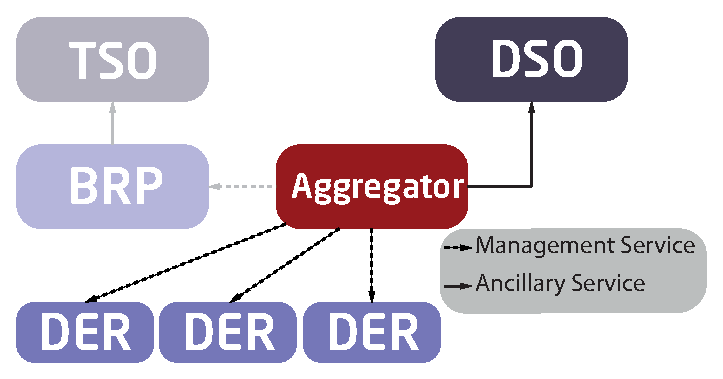
\includegraphics[width=0.7\textwidth]{isgt2014/system.eps}
		\caption{The setup of the power system with DSM. Note that the Aggregator can either be an independent entity or can be a role inside a BRP.}\label{fig:systemarch}
	\end{figure}
	
%	The objective of a DER is to satisfy the needs of its owner. The Aggregator provides the DER owners with an asset management service that ensures the QoS to customers is adequate. Providing services to the grid is only a secondary (and optional) function of the DER, which the Aggregator must take advantage of within the constraints of the primary function. 
	
%	The power consumption of DERs varies greatly depending on the daily routines of their owners and the meteorological conditions. Due to the varying load size, behavior and distributed nature of the DERs, the Aggregator must be able to evaluate if its control algorithms are capable of providing ancillary services and asset management satisfactorily.

	% subsection asset_management_service (end)
	
	\subsection{Control Performance Assessment}
	There is a field of theory on evaluation of controllers: Control Performance Assessment (CPA). Applications of this theory are found mostly in the process industry; for a thorough overview of its applications we refer to \cite{Jelali,Green}. 

		Typically, CPA methods fall within two approaches. One approach, first introduced in \cite{Harris1989}, is to benchmark controller performance against a theoretical optimum, while taking the stochasticity of the system into account. The second approach is to benchmark against deterministic properties the closed-loop system must have, e.g. settling time and steady-state error \cite{Astrom}. In both cases, the index is usually scaled such that:
\begin{equation}
	\zeta = \frac{J_{opt}}{J_{act}},\label{eq:astrom}
\end{equation}
where $J_{opt}$ is the theoretical optimal (minimum) value of the performance criterion \emph{J} (which is usually impossible to achieve in reality), and $J_{act}$ is the actual measured value of the criterion. Since $J_{opt}<J_{act}$, then $\zeta \in [0,1]$. 
		%Given that the requirements of service delivery are easily translated into time-domain deterministic measures, this work presents a deterministic approach. Using the concepts presented in this section, the performance index is defined in the next section.
%In the following, we propose the application of CPA concepts to DSM.

		According to \cite{Green}, performance criteria used to evaluate a controller usually fall within three categories: Quality, Reliability, and Energy. Quality and reliability are concepts that can be directly related to ancillary service provision. The interpretation of energy-related criteria may be suitable for asset-management purposes but is considered out of scope in this work.% The quality of the control performance is measured by the QoS it provides, both towards the system operators and towards its customers. Reliability is measured as how many times the controller provides a QoS outside the specified limits.

\section{DSM Performance Assessment} % (fold)
\label{sec:index}
We identify four requirements for performance assessment of DSM:
\begin{itemize}
	\item[R1] Provide a \emph{quality} measure normalized to the contractual requirements (bounds) of a service. By normalizing the quality measure to the bounds, the \emph{QoS} value for both ancillary services and asset-management services will have comparable dimensions.
	\item[R2] The measure should be normalized with respect to time.
	\item[R3] Provide a \emph{reliability} measure in relation to service non-delivery.
	\item[R4] Each service must have a separate, individually verifiable, measure. For example, to evaluate service delivery w.r.t. ancillary-service delivery, the asset-management quality is irrelevant.
\end{itemize}

To satisfy these requirements, we propose a performance index quantifying the quality of ancillary services and asset-management services, and a non-delivery counter (NDC) which increases every time the QoS is out of bounds. Normalization is based on a scaling factor modeled after the contractual limits of the respective service. The limits are defined via a contract with the entity requesting the service. Thus, the performance index is specifically designed to evaluate how well the service provision conforms to the contractual boundaries.
	%The formulation of a performance index transforms the service requirements of the Aggregator into a single computable quality measure. %The index presented here is defined for post-simulation analysis, and represents the performance of the control algorithm over the whole time horizon. 
	\subsection{Definition of the performance index}
	In previous sections we have defined the concept of QoS as a deviation, $e(t)$, from a contracted behavior. Since there is a contractual limit on the allowed deviation, the error is normed to be a percentage of this limit such that:
	\begin{equation}
		QoS_{s}(t)=|e(t)|C_{s}(t); \quad  QoS_{s}(t)\in [0,1]
	\end{equation}
	where \emph{s} is either \emph{AS} for ancillary service or \emph{AMS} for asset-management service, and $C_s(t)$ is the corresponding normalization factor derived from the service model. When $QoS_{AS}(t) \geq 1$, the measure for reliability NDC is increased. %For the ancillary services this is simply expressed as $QoS_{AS}(t) = e(t)_{AS}$ while the expression for the asset management service is $QoS_{AM}(t) =\sum_{k=1}^M e(t)_{AM}$.

	Using the square root of the Integral Square Error index (i.e. the 2-norm, as defined in e.g. \cite{Skogestad}), the following performance criterion is defined for service delivery seen from the Aggregator perspective:
	\begin{equation}
		%\text{J}=\sqrt{\int_{0}^{N}\left( \sum_{k=1}^M |e(t)_{AM,k}C_{AM}|^{2}+|e(t)_{AS}C_{AS}|^{2}\right)dt} 
		{J}(N)=\sqrt{\int_{0}^{N}\left( \sum_{k=1}^M {QoS}_{AMS,k}(t)^{2}+{QoS}_{AS}(t)^{2}\right)dt} 
	\end{equation}
where ${QoS}_{AM,k}(t)$ and ${QoS}_{AS}(t)$ are the time-dependent measures of service quality for the asset-management service and the ancillary service, respectively. The units controlled by the Aggregator are denoted by the index \emph{k}, the unit portfolio is of size \emph{M}, and \emph{N} is the time horizon over which the services are provided. %Finally, $Q_D$ and $Q_U$ are scaling factors that convert the errors into percentages so that $e(t)_D$ and $e(t)_U$ are comparable. 
While the index~\eqref{eq:astrom} benchmarks the actual performance criterion against a theoretical minimum, we benchmark it against the worst case scenario $J_{max}$, such that the performance index is given by:
	\begin{equation} 
		\eta = \frac{J_{act}(N)}{J_{max}(N)}\label{eq:eta}
	\end{equation}
	where $\eta \in [0,1)$ for a valid service delivery and for which values close to zero represent good performance of service delivery. If $\eta \geq 1$ the Aggregator does not perform according to its service contract.
		
		Normalization with respect to time is achieved when benchmarking against $J_{max}(N)$, since $J_{max}(N)$ is estimated by integrating over the service delivery period. Contrary to index \eqref{eq:astrom}, which gives an intuition of how close performance is to the optimum, index \eqref{eq:eta} gives an intuition of how far performance is from the worst case scenario. The index is designed this way because the theoretical optimum of service delivery is $J_{opt}=0$, i.e. no error in service delivery.
	%It must be noted that the performance criterion only measures the permissible error defined in the contract of the service (the service quality), and service non-delivery (the service reliability) is measured separately. Therefore, whenever the algorithm performs outside the established limits, then $J(t)_{act}=J(t)_{max}$ and a non-delivery counter is increased.
	\subsection{Calculating the index}\label{sub:modelcalc}
	Having defined what the performance index measures, we will proceed with establishing how to obtain the required values to estimate the index. Calculating the performance index requires the following steps:
	% the maximum permissible error ($J(t)_{max}$) of the service requires two steps:
		\begin{enumerate}
		\item Identify and model the service requirements and errors in service provision, giving the scaling factor $C(t)_s$.
			\item Estimate $J_{act}(N)$.
			\item Calculate \emph{J(N)} for operation on the requirement boundaries ($J_{max}(N)$).
			\item Calculate $\eta$ by benchmarking $J_{act}(N)$ with $J_{max}(N)$.
		\end{enumerate}	
		
	For the first step, the service requirements must be defined and translated into measurable errors. For some services, the error can be stated as a tracking error, e.g. $e=y_{ref}-y_{meas}$. In other cases, service requirements are defined by operation within bands, which may lead to an error defined as:
	\begin{equation}
	e(x)= \left\{ \begin{array}{l l}
	x_{min} - x & \quad \text{ if } x \leq x_{min}\\
	0 & \quad \text{ if } x_{min} \leq x \leq x_{max}\\
	x - x_{max} & \quad \text{ if } x \geq x_{max}
	\end{array} \right.
	\end{equation}
	This step is a service-specific problem and is non trivial.

	The second step requires computing $J_{act}(N)$ using measurement data from the unit portfolio. This can be a challenge for evaluation in field deployment. In this paper it is assumed that the measurement data is available, either through a DSO or a third-party metering company.	
	
		%The actual performance of the aggregation algorithm can be found through two different methods:
%\begin{itemize}
	%\item On-line monitoring -- This method brings the added benefit of being able to use the index for performance monitoring and diagnosis at runtime, but the downside of being communication intensive.  
	%\item Post-delivery analysis -- This method is less communication intensive, but does not permit to take remedial actions at run time if a aggregation controller is not working as expected.
%\end{itemize}
%	Usually services have some acceptable error (see Sec.~\ref{sub:ancillary}) which can be interpreted as the hard boundaries for the service delivery.
	The third step requires the calculation of \emph{J(N)} along the contractual boundaries for service delivery, in this way, the maximum allowed error is found for the service. The boundaries are based on the service models presented in the first step. By adding the maximum permissible error for all services, $J_{max}(N)$ is obtained. 
	%Normalizing the performance measure with the $J_{max}$ gives an intuitive value of the performance of the control algorithm.
	The following subsection present an example of how to determine $J_{max}(N)$.

	\subsection{An example: DSO Service PowerMax}\label{sub:example}
	For demonstration purposes, in this section $J_{max}(N)$ for the PowerMax service is calculated. 
	Typically, the service will be contracted several months ahead of the actual delivery. The activation schedule (On and Off triggers), the maximum power cap ($P_M$), the maximum duration of the service per activation ($T_M$), and the quality of service (\emph{QoS}) are defined when contracting the service. The contract is valid for a period of several months, where the Aggregator is obliged to follow the established schedule.

	The limits specified for the QoS\cite{FLECH} of the PowerMax service are presented here: 
	\begin{itemize}
		\item Deviation from On trigger: $\pm$ 15 min. per day
		\item Deviation in size of service (dependent on $P_M$): Max. $\pm 5\% P_M$  
		\item Acceptable no. of unsatisfactory activations(non-delivery): $\text{NDC} = 4$
	\end{itemize}

A graphical representation of these service requirements is depicted in Fig.~\ref{fig:servicereq}. It is clear that the maximum acceptable error in service delivery is the shaded area. Note that the limit for non-delivery of service during the first 15 minutes of activation is dotted due to the fact that non-delivery is not counted during this period. The specifications for counting unsatisfactory activations are not clarified in \cite{FLECH}, so it is assumed that breaking the QoS limits on one sampling period counts as one non-delivery. In the case where the service is not respected in three consecutive (or non-consecutive) sampling periods, $\text{NDC}=3$.

For example, in the case where  $P_M = 5\,kW$, $T_M=4\, h$ and the power is measured once an hour, $J_{max}(N) = 2$, as it represents the square root of the square of the maximum (when $J_{act}(N)=1$) permissible error over 4 hours.
\begin{figure}[t]  % Find out how to send it to next column.
	\centering
	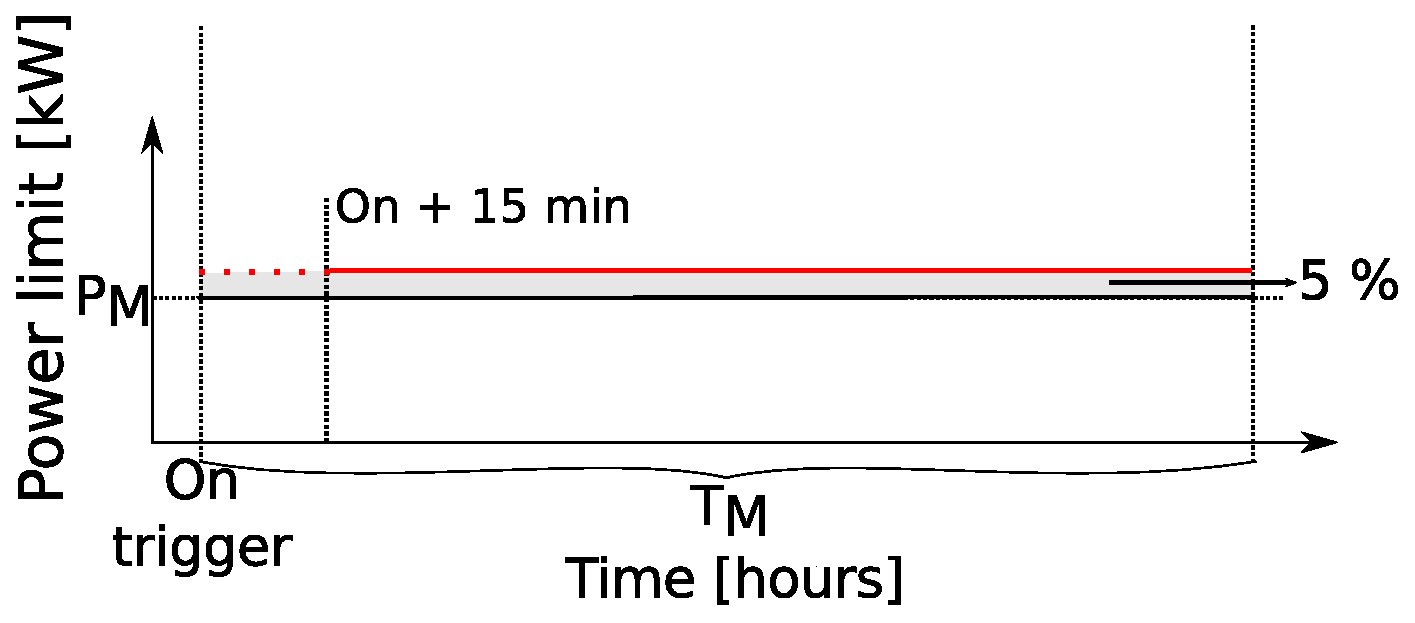
\includegraphics[width=2.5in]{isgt2014/drawing3.eps}
	\caption{The PowerMax service requirements, where the red line represents the boundaries for the permissible error, and the shaded area represents the error in service delivery, which is within the limits established in the QoS. }\label{fig:servicereq}
\end{figure}

	
% section the_performance_index (end)

\section{Case Study}
\label{sec:case}
This case study presents the aggregation of multiple flexible DERs via coordinated operation: 75 DERs installed in a suburban residential area, which are all connected to the same feeder leading to a 10/0.4 kV transformer. The transformer is rated to a maximum power flow of 200 kVA, which is sufficient under the current load circumstances, but will be a constraint in the future.

This case study addresses a scenario with high electric-vehicle (EV) penetration, low photo-voltaic (PV) penetration and electric space heating in all households. Furthermore all DERs connected to the same LV feeder offer their flexibility to the same Aggregator. Then, the proposed performance index for service provision is evaluated for two different aggregation control algorithms: Centralized soft Model Predictive Control (C-MPC) and Distributed soft Model Predictive Control (D-MPC).

\subsection{The reference case: without units coordination}
In this section we make a scenario hypothesis for year 2050 regarding PV and EV penetration in a distribution feeder in a rural area and present simulation results. The following units are connected to the LV transformer:
\begin{itemize}
\item 40 buildings with electric climate control: resistive space heating with maximum load of 10 kW and air conditioning with a maximum load of 5 kW.
\item 20 large EVs, with a battery size of 25 kWh, 11 kW.
\item 10 small EVs, with a battery size of 14 kWh, 3.3 kW.
\item 5 PV (polycrystalline) installations of 6 kW rated power each.
%\item 5 Li-On support batteries for local energy storage: 10 kWh, 2 kW each (95\% round trip efficiency). 
\end{itemize} 

The PV installations provide forecasts of the production for one day ahead. To simulate uncertainty in the forecasts, Gaussian noise has been added to real data of PV production according to:
\begin{equation}
	{P_{PV-F,t}} = {P_{PV-T,t}} + {v_t},\quad {v_t} \sim N\left( {0,\alpha  \sqrt {{P_{PV-T,t}}} } \right)\label{eq:pvprod}
\end{equation}
where $P_{PV-F,t}$ is the forecasted PV power production at time $t$, and $P_{PV-T,t}$ is the actual power production at time $t$ (from historical data). The term $\alpha$ is an uncertainty factor, which defines the variance of the noise as a percentage of the actual PV production, e.g. $\alpha = 0.1$ corresponds to a $10\%$ forecast error. Uncertainty in solar radiation and ambient temperature are modeled in the same way. The actual power production time-series used in this case covers the same days as \cite{costanzo2013coordination}.

The load related to households is divided into climate control (flexible load) and everything else (non-flexible load). The building climate control is operated on MPC basis for minimum deviation from the temperature set point. Regarding the non flexible household loads, a five-day (one-hour-sampled) profile of the non-flexible load of 40 households is depicted in Fig.~\ref{fig:nonflexible}.

\begin{figure}[t]  
	\centering
	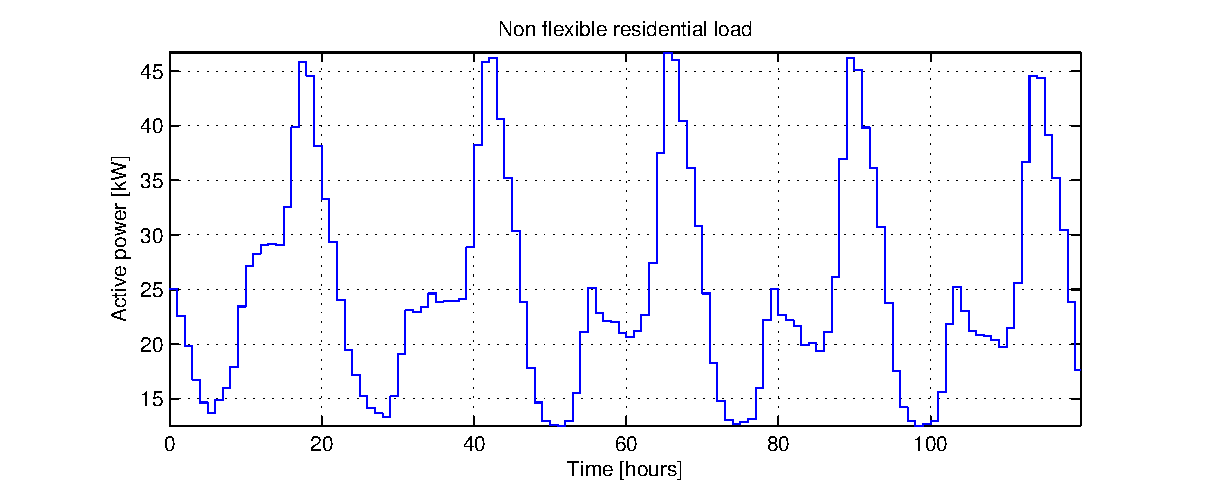
\includegraphics[width=\textwidth]{isgt2014/nonflexload.eps}
	\caption{The non-flexible load of the households under the transformer. The sample is statistically representative of Danish households.}\label{fig:nonflexible}
\end{figure}

The EVs leave the charging station at a uniform randomly distributed time between 6:00  and 8:00, and are plugged again at a uniform, randomly distributed time between 16:00 and 18:00. The EVs operate on dumb charging, i.e. they try to fully charge as soon as they are connected to the grid.  %The energy price is the same for all the units within the same cluster.
By running a simulation of the described scenario without units coordination, the results shown in Fig.~\ref{fig:referencecase} are obtained.

\begin{figure}[t]  
	\centering
	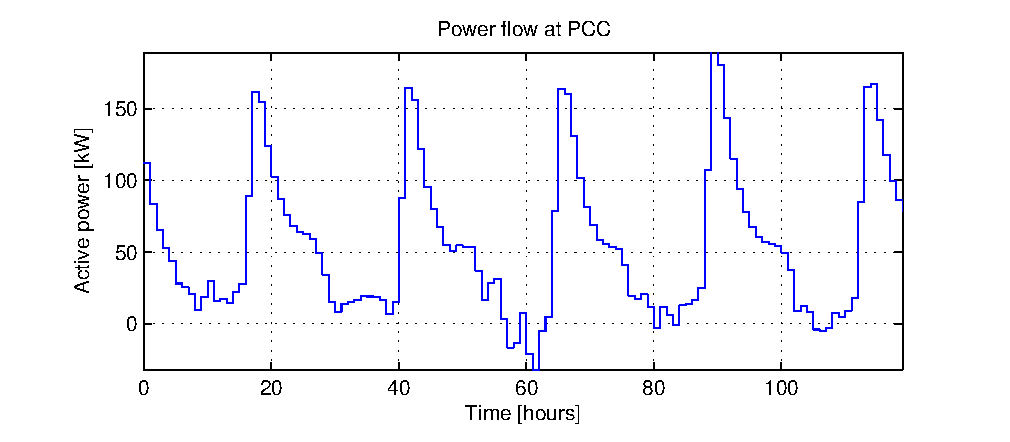
\includegraphics[width=\textwidth]{isgt2014/referencecase.eps}
	\caption{Aggregated power flow at the point of common coupling for the reference case units without coordination: Demand Response based on day-ahead energy price.}\label{fig:referencecase}
\end{figure}

EVs operating on dumb charging can cause peak consumption up to 190 kW at the point of common coupling (PCC). Given that the transformer capacity is 200 kW and it is customary to reserve 30\% of the transformer capacity for emergency operations \cite{Engel}, the DSO aims at keeping the load below 140 kW and limiting the inverse power flow at the substation. Thus, the DSO can sign a contract for PowerMax service (see Sec.~\ref{sub:example}) with an Aggregator which, at any time, operates Demand Response via Direct Load Control (DLC)~\cite{kosek2013overview} in order to limit the power flow at the transformer. The maximum capacity available at the transformer is therefore 140 kW for direct power flow and -10 kW for inverse power flow.

The rest of this section presents the C-MPC and D-MPC formulations. For the formulation of the mathematical models we refer to~\cite{6345063} for the battery model and to~\cite{Bacher20111511} for the building space heating model (modified, as proposed in~\cite{costanzo2013coordination}). For the modeling of the services, we apply the method described in Sec.\ref{sub:modelcalc}. A discussion on the simulation results concludes this section.
\subsection{The Centralized Model Predictive Control scheme}
\begin{figure}[t]  
	\centering
	\subfloat[The setup of the Centralized MPC scheme.]{\includegraphics[width=1.0\textwidth]{isgt2014/centralized.eps}\label{fig:centralized}}
\\
\subfloat[The setup of the DMPC scheme as seen in \cite{costanzo2013coordination}.]{\includegraphics[width=1.0\textwidth]{isgt2014/blackboard.eps}%
\label{fig:blackboard}}
\caption{The setup of the two Aggregation algorithms to be compared.}\label{fig:systemsetup}
\end{figure}
In this scheme the Aggregator contains the control algorithm to centrally manage all the units in its portfolio (Fig.~\ref{fig:systemsetup}(a)). Since the Aggregator optimizes its portfolio's consumption through MPC, it has detailed knowledge of the state and dynamics underneath.
The units portfolio is the same as of the reference case. The C-MPC control problem is formulated as quadratic optimization with soft constraints (as seen in e.g. \cite{prasath2009a}):
{%\footnotesize
{\begin{subequations}\label{Eq: building_MPC}
\begin{align}
& \min\limits_{u_t,\vartheta_t} \; {J} = \sum\limits_{t = 1}^N {\left[ {\left\| {y_{t} - r_t} \right\|_Q^2} + {\rho}\vartheta_t + \psi \gamma_t \right]} \label{Eq: building_MPC_objective}\\
& subject \; to: \nonumber \\
& x_{t + 1} = Ax_t + B u_t + Ed_t\label{Eq: building_MPC_constraint1}\\
& y_t = {C}x_t +Du_t \label{Eq: building_MPC_constraint2}\\
& u_{\min ,t} \le u_t \le u_{\max ,t} \label{Eq: building_MPC_constraint3}\\
& y_{\min ,t} - \gamma_t \le y_{t} \le y_{\max ,t} + \gamma_t \label{Eq: building_MPC_constraint4}\\
& {PCC_{\min ,t}} - \vartheta _t \le u_t \le {PCC_{\max ,t}} + \vartheta _t \label{Eq: building_MPC_constraint5}\\
& \vartheta_t,\gamma_t \ge 0 \label{Eq: building_MPC_constraint6}
%& \gamma_t \ge 0 \label{Eq: building_MPC_constraint7}
\end{align}
\end{subequations}}}
where $r_t$ and $y_t$ are the output reference and system outputs (internal house temperature and battery state of charge) respectively over the prediction horizon $t=1..N$, $\psi$ is the weight for output soft constraints, with $\gamma$ being the corresponding slack variable, and $\rho$ penalizes the \emph{power over max} defined in Eq.~\ref{Eq: building_MPC_constraint5}. Since this MPC controller is centralized, the state space system matrices in Eq.~\eqref{Eq: building_MPC_constraint1} and Eq.~\eqref{Eq: building_MPC_constraint2} are formed by block diagonal-adding each of the systems' respective matrices. With the set of units $\mathcal{S}=\{1..N\}$, it follows:
%
{ \begin{equation}
\begin{array}{l}
x = \left[ {\begin{array}{*{20}{c}}
{{x_1}}\\
{{x_j}}
\end{array}} \right],u = \left[ {\begin{array}{*{20}{c}}
{{u_1}}\\
{{u_j}}
\end{array}} \right],d = \left[ {\begin{array}{*{20}{c}}
{{d_1}}\\
{{d_j}}
\end{array}} \right],y = \left[ {\begin{array}{*{20}{c}}
{{y_1}}\\
{{y_j}}
\end{array}} \right]\\
\\
A = \left[ {\begin{array}{*{20}{c}}
{{A_1}}&0\\
0&{{A_j}}
\end{array}} \right],\quad B = \left[ {\begin{array}{*{20}{c}}
{{B_1}}&0\\
0&{{B_j}}
\end{array}} \right]\\
\\
C = \left[ {\begin{array}{*{20}{c}}
{{C_1}}&0\\
0&{{C_j}}
\end{array}} \right],\quad D = \left[ {\begin{array}{*{20}{c}}
{{D_1}}&0\\
0&{{D_j}}
\end{array}} \right]\\
\\
E = \left[ {\begin{array}{*{20}{c}}
{{E_1}}&0\\
0&{{E_j}}
\end{array}} \right],\quad \vartheta  = \left[ {\begin{array}{*{20}{c}}
{{\vartheta _1}}\\
{{\vartheta _j}}
\end{array}} \right],\gamma  = \left[ {\begin{array}{*{20}{c}}
{{\gamma _1}}\\
{{\gamma _j}}
\end{array}} \right]
\end{array}
\end{equation}}
%\normalsize
where the index $j \in \mathcal{S}$ and the system in Eq.~\eqref{Eq: building_MPC_constraint1} and Eq.~\eqref{Eq: building_MPC_constraint2} is extended with all the units belonging to the set $\mathcal{S}$.
\subsection{The Distributed Model Predictive Control scheme}
%The computational effort for solving centralized MPC problems generally grows at a super-linear rate with the number of state variables involved. The exact order is problem-specific and depends on the coupling between the state variables as well as the chosen solving method. Decomposing the C-MPC problem into smaller MPC sub-problems that can be solved independently and locally at the unit level helps in solving the curse of dimensionality. Convergence towards the overall goal is then achieved through a blackboard coordination mechanism, which ensures data exchange between the individual solvers.
In the D-MPC formulation, units within the same cluster retrieve the power plans of the other units, compute their own plan (over a prediction horizon) accordingly and publish it on a blackboard. Note that in this case study, in contrast to what has been proposed in~\cite{costanzo2013coordination}, the unit controllers have soft constraints on the outputs (temperature for buildings and State of Charge (SOC) for batteries and EVs). In this algorithm, as soon as the units publish their consumption plan, the available power at the PCC decreases in such a way that the subsequent units communicating with the blackboard tend to adjust their plan accordingly. After a negotiation period the units are entitled to operate according to the power plan that has been published in the blackboard for the next time frame. Figure~\ref{fig:systemsetup}(b) shows the configuration for the D-MPC. This is an example of transactional control \cite{kosek2013overview}, where the unit power consumption is negotiated.
\subsection{Comparison and discussion of results} \label{sub:comparison}
Certain assumptions have been made with regards to controllers:

%\begin{itemize}
The EVs are preferably kept operating in the range $SOC = [0.2,0.9]$ due to battery life concerns\cite{6345063}, although it is possible to operate in $SOC=[0.0,1.0]$.
The comfort band for the households lies in the band $T_{ref}=22{}^{\circ} C \pm 1{}^{\circ} C $. The concept of non-delivery is not used in the asset-management services, but the absolute boundaries for user-comfort bands lie on $T_{ref}=22{}^{\circ} C \pm 1.5{}^{\circ} C $.

The required PowerMax service is of $P_M = 90kW $ each day in the periods of 16:30 to 20:30.
The time sampling of the simulation is of 15 minutes and the power plans are computed for a horizon of 23 hours (i.e. the MPC prediction horizon).
%\item The EVs are not available during the day, when they are used for transport, and in these periods the MPC for the EV is inactive.
The EVs are not capable of providing Vehicle-to-Grid (V2G) services, i.e. EVs only charge.

%\end{itemize}
These assumptions lead to the results presented Figs.~\ref{fig:dmpcsimres}-\ref{fig:pccsimres} and Tables \ref{tab:comparison}-\ref{tab:days}.
The following conclusions can be made:

1) from Figs.~\ref{fig:dmpcsimres} and \ref{fig:cmpcsimres} it can be seen that both controllers are quite good at staying within the QoS limits of the DSO and EV owners, which can be seen in the fact that none of the controllers have non-delivery and $\eta$ is small. It is clear that the value of $\eta$ comes from the behavior of the household heating, where the C-MPC delivers a better quality service to end users than the D-MPC, although it might not be obvious from the figures. % Also, from Fig.~\ref{fig:pccsimres}, it is clear that the PowerMax service is delivered at all times.

2) controller performance is sensitive to prediction uncertainties, as can be seen in the varying values of $\eta$ depending on the uncertainty $\alpha$ (see Eq.~\eqref{eq:pvprod}), which is shown in Table~\ref{tab:comparison}.
	%\item By changing some of the different weights on the controllers, e.g. prioritizing the upwards service versus the downwards service, leads to different results it $\eta$ (this is not shown in the figures).

3) in terms of service provision, the C-MPC outperforms the D-MPC. This arises from the fact that the C-MPC has absolute control of all units and determines a global optimum.

4) due to the behavior difference between the local EV controllers in the D-MPC scheme, and the behavior of the C-MPC, the power consumption of the EV is very different (compare Fig.~\ref{fig:dmpcsimres}(b) and Fig.~\ref{fig:cmpcsimres}(b)). This also leads to a vast difference in the power flow at PCC (see Fig.~\ref{fig:pccsimres}).

5) from the values in Table~\ref{tab:days}, it can be seen that the values of $\eta$ are in the same order of magnitude when simulations are done for varying numbers of days. This is caused by the normalization of $J_{act}(N)$ over time (reflected in $J_{max}(N)$). This means $\eta$ evaluates the aggregation algorithm taking service provision time into account, and gives an overall assessment of the algorithm, dependent on the length of time the Aggregator must sustain the service provision. %An error in provision of a specific size will have less impact on $\eta$ if the service time is long. This makes sense since an error  

\begin{figure}[!t]
\centering
\subfloat[Households temperatures]{\includegraphics[width=1.0\textwidth]{isgt2014/DMPCalpha01/building2.eps}%
\label{fig:dmpchouse}}
\\
\subfloat[EV State of Charge]{\includegraphics[width=1.0\textwidth]{isgt2014/DMPCalpha01/EVs.eps}%
\label{fig:dmpcev}}
\caption{Simulation results for the D-MPC with $\alpha=0.1$}
\label{fig:dmpcsimres}
\end{figure}

\begin{figure}[!t]
\centering
\subfloat[Households temperatures]{\includegraphics[width=1.0\textwidth]{isgt2014/CMPCalpha01/buildings.eps}%
\label{fig:cmpchouse}}
\\
\subfloat[EV State of Charge]{\includegraphics[width=1.0\textwidth]{isgt2014/CMPCalpha01/EVs.eps}%
\label{fig:cmpcev}}
\centering
\caption{Simulation results for the C-MPC with $\alpha=0.1$}
\label{fig:cmpcsimres}
\end{figure}

\begin{figure}[!t]
\centering{\subfloat[Total power load for C-MPC]{\includegraphics[width=0.5\textwidth]{isgt2014/CMPCalpha01/PCC.eps}%
\label{cmpcpcc}}
\subfloat[Total power load for D-MPC]{\includegraphics[width=0.5\textwidth]{isgt2014/DMPCalpha01/PCC.eps}%
\label{dmpcpcc}}}
\centering
\caption{Power load at Point of Common Coupling for the controllable and non-controllable loads}
\label{fig:pccsimres}
\end{figure}

% increase table row spacing, adjust to taste
%\renewcommand{\arraystretch}{2.3}
%if using array.sty, it might be a good idea to tweak the value of
% \extrarowheight as needed to properly center the text within the cells
\begin{table}
\caption{Results of three-day simulation}\label{tab:comparison}
\centering
% Some packages, such as MDW tools, offer better commands for making tables
% than the plain LaTeX2e tabular which is used here.
\begin{tabular}{c|c c c c}
\hline
&\multicolumn{2}{c}{D-MPC} & \multicolumn{2}{c}{C-MPC} \\
\hline
$\alpha$ & 0.1 &0.2&0.1&0.2\\
NDC&0 &0 &0 &0\\
$\eta$&0.0075 &0.0160&0.0054&0.0153\\
\hline
\end{tabular}
\end{table}

\begin{table}
	\caption{D-MPC Performance over different simulation lengths}\label{tab:days}
	\centering
\begin{tabular}{c|c c c c c}
\hline
Days simulated & 1 & 2 & 3 & 4 & 5 \\
$\eta$ &0.0013&0.0018 &0.0082&0.0052&0.0062\\
\hline
\end{tabular}
\end{table}

	\section{Conclusion and Outlook}
	\label{sec:conclusion}
	Drawing inspiration from the field of Control Performance Assessment, this study proposes a performance index for the evaluation of control services for DER aggregation. The index is useful for the systematic evaluation of the adequacy of different control architectures providing ancillary services.
It was shown how the index is computed, and a case study was presented in which two different control algorithms were evaluated. The results were presented and discussed, showing that the C-MPC in this case is capable of providing a better QoS.
%Evaluation of aggregation algorithms is expected to be an important part of validation of Aggregators providing DSM. 
%	 As modelled in this paper, the index only gives a general idea of the performance of the control algorithm, but future work could include a method for differentiating the sources of high error.
	In order to do a successful evaluation of an aggregation algorithm, it is important that the QoS specifications of the future ancillary services are well defined. This is a challenge in itself since many of the ancillary services assume a production baseline, which is easy to establish in traditional generators, but proves to be difficult for small households (see e.g. \cite{Borenstein}). Research effort should be put into redefining ancillary-service requirements to suit DSM, taking into account the probabilistic nature of managing a large number of units.

 The evaluation of aggregation control algorithms is an important part of a general validation framework for Aggregators. Future work will include further development of this Aggregator validation framework, where controllers can be tested under different grid and communication network topologies, as well as a diverse set of fault scenarios.

\section*{Acknowledgment}

The authors acknowledge the financial support of iPower (www.ipower-net.dk).
The authors thank Shi You from DTU Elektro for providing data for the non-controllable loads.


